\chapter{DCM for Evoked Responses\label{Chap:DCM_ERP}}

This chapter demonstrates an example of Dynamic Causal Modelling for
Evoked Responses, based on the analyses as detailed by Tyrer, \emph{et
al}. (Tyrer \emph{et al.}, 2020). The purpose of the following analyses
is to estimate the effective connectivity between sources of activity in
the brain, in the context of a visual repetition memory paradigm.

In this chapter, the example here uses pre-existing data from a DCM for
EEG study in Alzheimer's disease patients and healthy aged controls
(Tyrer \emph{et al.}, 2020). The key aims of this study were to
investigate how inter-regional connectivity and within-region dynamics
during implicit and explicit memory processing are implicated in
Alzheimer's disease, and to examine whether such connections in the
right hemisphere provided compensation during these memory tasks. We
hypothesized that hierarchical left-hemisphere specific connections may
be weakened in the Alzheimer's patient cohort compared with healthy aged
controls.

One of the paradigms used in this study was a visual recognition task.
Participants completed an encoding phase in which they were shown 100
images of nameable objects and were asked to press a button as they
covertly named the object in the image. They then underwent EEG
recording and during EEG recording they were presented with 100 images
again, but 50 images were novel images, and 50 images were repeated from
the encoding phase. These were presented in a random order, and
participants had to register with a button press either whether or not
they thought they had seen the image before. Therefore, this task
consists of two different conditions: the novel image condition and the
repeated image condition. The single-participant data used here is that
of a healthy aged control participant in this visual recognition task.

DCM is a hypothesis-driven method, and can be used to test specific
hypotheses about the activity between sources in a network rather than
simply being limited to asking questions about the strengths of the
sources individually. DCM estimates effective connectivity as opposed to
structural or functional connectivity, which is context-dependent.
Rather than asking questions such as "How does one source increase the
activity in another source?", with DCM you can ask context-dependent
questions such as "How does one source have an influence over another
source in a particular condition within a task?". DCM estimates this
effective connectivity both within and between sources of activity, and
these connections are examined in the context of regional activity
changes, and also in a task-dependent fashion, so you can derive the way
in which any experimental conditions that forms part of a task recruit
or modulate any specific connections.

A further characteristic of DCM is that, through inversion of the model
according to a Variational Bayesian scheme, this yields an approximation
to the log-model evidence, which one can use to compare alternative
models of the same data and make statistical inferences about which
model best represents the data, i.e. has the highest model evidence.

\section{Data}

For this example we will use the pre-processed (band-pass filtered,
epoched, artefact-corrected) EEG dataset\footnote{DCM for ERP dataset: \url{https://www.fil.ion.ucl.ac.uk/spm/data/dcm-erp/}} saved in the files:

\begin{verbatim}
mfaeffspmeeg_examplecontrolsubject.mat
mfaeffspmeeg_examplecontrolsubject.dat
\end{verbatim}

Three-dimensional source reconstruction and coregistration are also
necessary for DCM for ERPs, so these steps should be performed in
advance of DCM model specification.

\section{Starting SPM for EEG}

First, ensure that the main SPM directory is in your \matlab\ path. Start
SPM 12 and select the M/EEG button, or type \texttt{spm eeg} in the command line.
This opens the SPM graphical user interface (GUI).

\section{Constructing Your DCM}

Once you have opened the SPM-GUI, you will see that the window is split
into four main sections (from top to bottom): `\emph{Temporal
pre-processing}', `\emph{Spatio-temporal modelling}', `\emph{Model
specification, review and estimation}', and `\emph{Inference}'. The
button which opens the DCM GUI can be found on the right side of the
`\emph{Spatio-temporal modelling}' section, which is second from the top
in the SPM window. This opens a new graphics window, containing all the
options required for you to specify your DCM (Figure~\ref{dcm-erp:fig:1}).

The DCM GUI consists of five sections: section one allows you to load
and save existing DCM files, and also select which type of model you
want to apply; section two, `\emph{Data and Design}', is for selecting
your data; section three, `\emph{Electromagnetic Model}', allows the
specification of the spatial forward model; section four,
`\emph{Neuronal Model}', is for specifying the connections within your
model and inverting your DCM, and the final section contains additional
buttons for viewing your results and conducting Bayesian Model Selection
(BMS), which we will cover later.

Before the model can be specified, you must first select the data you
wish to use for the model and progress through the sections in the fixed
order laid out in the GUI, due to dependencies across each section, i.e.
data selection \textgreater{} electromagnetic model \textgreater{}
neuronal model. You can move both forward and backward through the
sections by clicking the forward (\textbf{\textgreater{}}) and backward
(\textbf{\textless{}}) arrows respectively, and options within each
section can be specified in any order.

\begin{figure}
\begin{center}
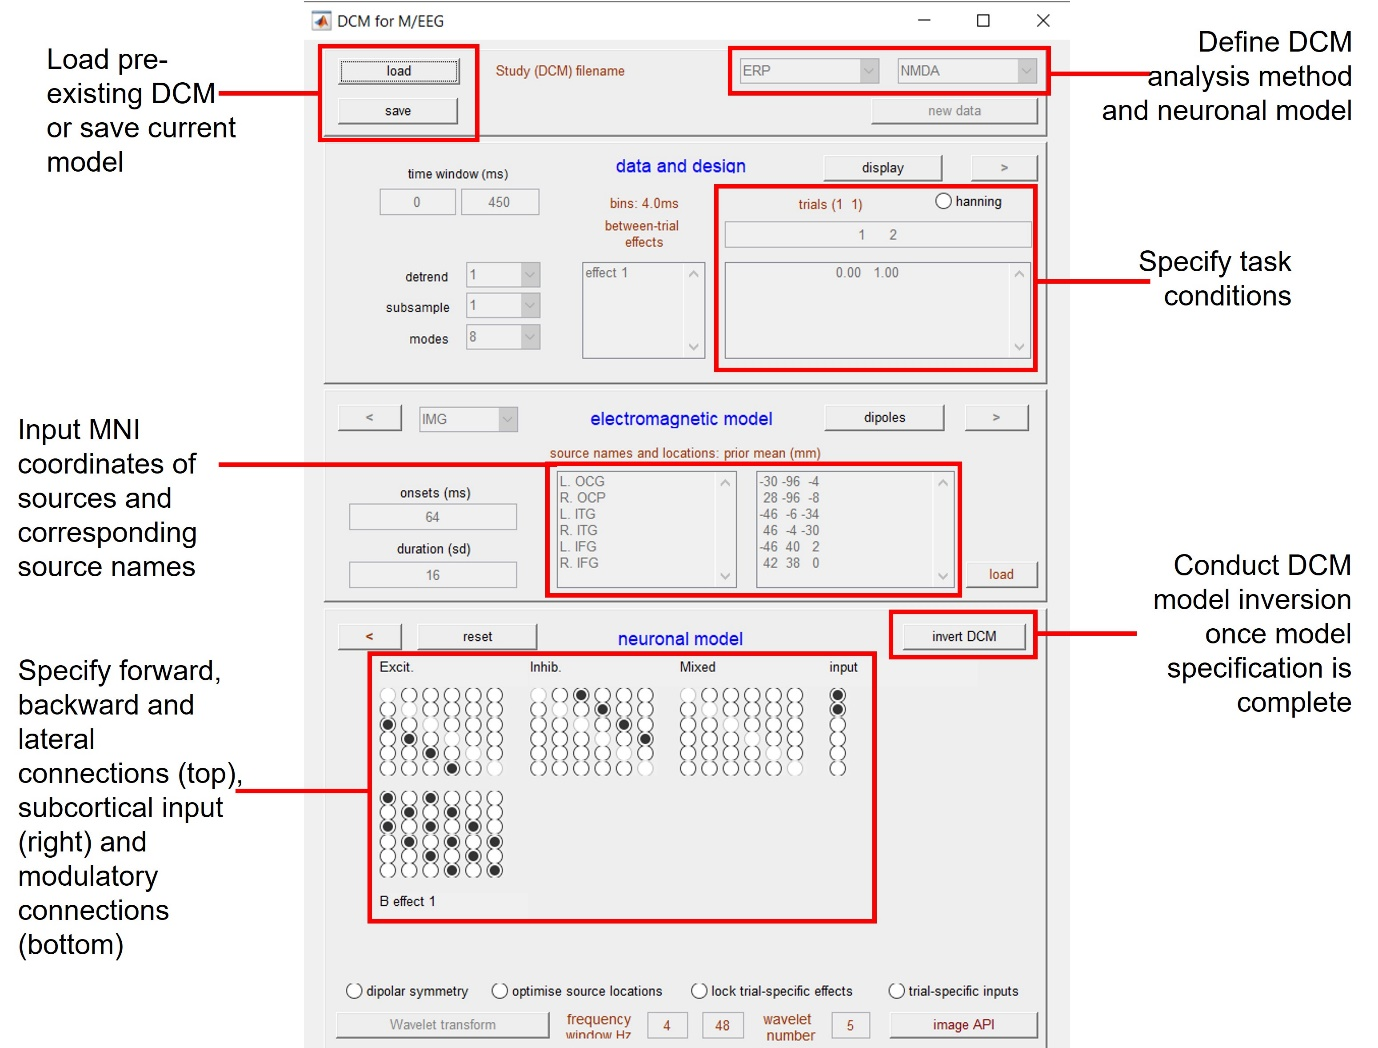
\includegraphics[width=6.26806in,height=4.76458in]{dcm_erp/figures/DCM_user_interface.png}
\caption{\em DCM user interface, configured for model inversion of the
six-source model with full B effect matrix for modulatory connections on
all connections in the model. To specify and invert your model, you must
specify each component in the correct order, from `\emph{Data and
Design'}, to `\emph{Electromagnetic Model'}, to `\emph{Neuronal Model'}.\label{dcm-erp:fig:1}}
\end{center}
\end{figure}

\subsection{Load, Save and Model Selection}

Starting with the first section in the DCM window, you can load a
pre-existing DCM into the GUI by clicking `load', or save a DCM you are
currently working on by clicking `save'. You can save and load your DCM
at any point during this specification process.

On the right side of this first section are two drop-down menus: the
leftmost menu defines the type of DCM analysis that you wish to conduct.
The default option is event-related potentials (ERP), i.e. DCM for
evoked responses, Alternatively you could select DCM for induced
responses (IND), cross-spectral density (CSD), neural field model (NFM),
time-frequency model (TFM), or phase coupled responses (PHA). For this
example we want to conduct DCM for evoked responses, so select the
default option: ERP.

The rightmost drop-down menu allows you to select the type of neuronal
model you wish to use. The default is once again ERP; other options are
sensory evoked potential (SEP), canonical microcircuit (CMC), local
field potential (LFP), neural mass model (NMM), mean field model (MFM),
canonical microcircuit model (CMM), NMDA, CMM including an NMDA receptor
model (CMM\_NMDA), and neural field model (NFM). For this example,
select NMDA. This neuronal model consists of a conductance-based neural
mass model with three cell subpopulations, and includes a model of the
NMDA receptor (Moran \emph{et al.}, 2011). The cell subpopulations
consist of pyramidal cells (extra-granular cortical layers), inhibitory
interneurons (extra-granular layers), and spiny stellate cells (granular
layers).

Beneath these drop-down menus, click the button `new data' to load your
data and select the data file mfaeffspmeeg\_examplecontrolsubject.mat.
Data files will generally contain epoched data with multiple trials per
condition. All data must be in SPM format to be used in DCM inversion.

\subsection{Data and Design}

In the next section below, `Data and Design', you can define the
peristimulus time window that the DCM will cover. In this example, by
entering 0 in the left box and 450 in the right box, we select the time
window 0-450 ms relative to the stimulus onset.

You can then specify the between-trial effects. In this task there are
two conditions: novel images and repeated images. The text box on the
right allows you to enter the trial indices of evoked responses in the
data file you have selected. For the two conditions in this task, enter
1 and 2 in the box, corresponding to `novel' and `repeated' trials,
respectively. To see which index is assigned to which trial condition,
type into the command line:

\begin{verbatim}
D = spm_eeg_load(`mfaeffspmeeg_examplecontrolsubject.mat');
D.condlist
\end{verbatim}

This will display the list of condition labels and their associated
indices. SPM should therefore display the following:

\begin{verbatim}
ans =

`novel' `repeated'
\end{verbatim}

indicating that index 1 corresponds to the presentation of novel images
and index 2 corresponds to the presentation of repeated images. The
default name of `effect 1' will be assigned to this effect by clicking
somewhere outside the text box, and will appear in the larger leftmost
text box.

The `detrend' option allows you to remove any low-frequency drifts at
the sensor level. Use this option to select the number of discrete
cosine transform terms you would like to remove. However, if you do not
wish to apply this, select the default value of 1 to simply remove the
mean. Similarly, the 'subsample' option defines the factor used to
down-sample the time bins. Here, this option can be left as the default
value of 1. The third option, `modes', allows you to define how many
frequency modes to model in your data. The modes essentially describe
the principal components of the data in sensor space. Generally, most of
the physiologically relevant activity is encompassed by the first few
modes, and the remaining modes just contain noise. The fewer modes you
use, the quicker the DCM model inversion will be. Therefore, you might
wish to run a DCM with a relatively large number of modes, and then see
how many of the later modes contain relevant/important activity and how
many contain noise. You might then run the model inversion again with a
reduced, optimised number of modes. The default number of modes is 8,
and for this example you can leave the number of modes as 8.

By clicking the 'Display' button on the top right, you can visualise the
different observed responses for the novel condition (top row) and for
the repeated condition (bottom row) in a separate graphics window
(Figure~\ref{dcm-erp:fig:2}). This displays the evoked responses for the two
conditions you specified: each line in the left-hand plots represents
the activity of a single channel. Visualising the data in this way is
useful for determining your choice of time window and your selected
detrending/subsampling options. You can change these options and click
`Display' again to see how changing these options affect the plots. To
move onto the next section in the GUI, click on the forward arrow
(\textgreater{}) on the right and this allows you to specify the
electromagnetic model.

\begin{figure}
\begin{center}
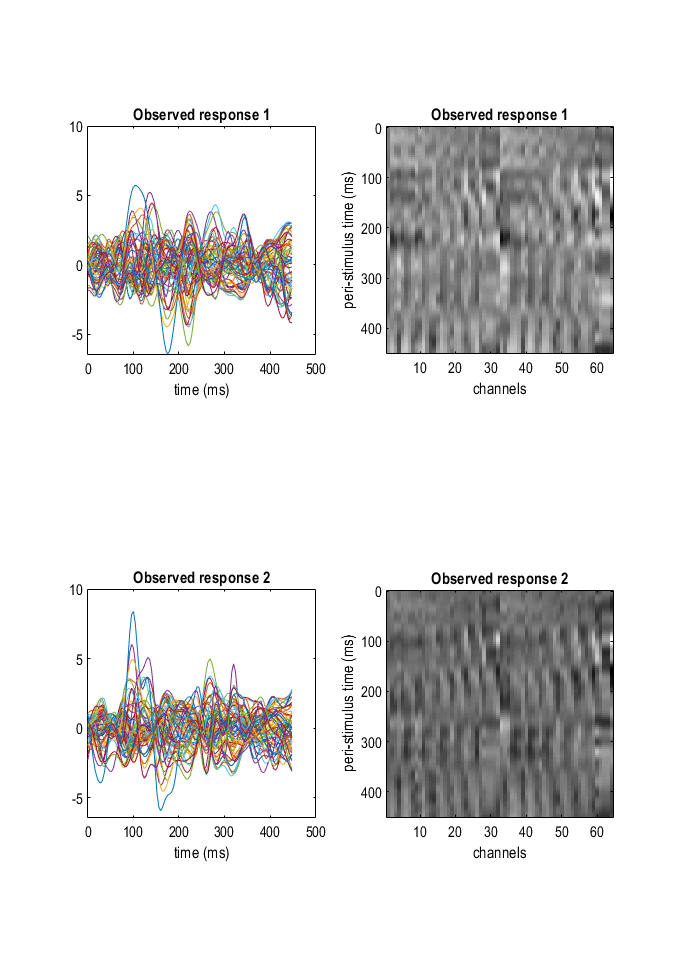
\includegraphics[width=4.54639in,height=6.02062in]{dcm_erp/figures/evoked_responses.png}
\caption{\em Evoked responses for the novel (top) and repeated (bottom)
conditions, following specification of the `\emph{Data and Design}'
section.\label{dcm-erp:fig:2}}
\end{center}
\end{figure}

\subsection{Electromagnetic Model}

In this section, you can specify the spatial model of the evoked
responses. With DCM for ERPs, there are four different options for how
to `spatially model' these evoked responses. This includes using a
single equivalent current dipole (ECD) for each source; applying a patch
on the cortical surface (IMG); or not using a spatial model and instead
treating each individual channel as a source (LFP). For this example,
select IMG.

By selecting IMG, you must then specify the prior source locations in
MNI space (i.e. in mm in MNI coordinates). This would also be the case
for DCMs using ECD. To specify source locations, you must enter a list
of source names in the large box on the left, and the corresponding MNI
coordinates in the large box on the right.

In the left large text box, enter:

\begin{verbatim}
L. OCG
R. OCP
L. ITG
R. ITG
L. IFG
R. IFG
\end{verbatim}

In the right large text box, enter:

\begin{verbatim}
-30 -96 -4
28 -96 -8
-46 -6 -34
46 -4 -30
-46 40 2
42 38 0
\end{verbatim}

These sources correspond to the left Occipital Gyrus, right Occipital
Pole, left Inferior Temporal Gyrus, right Inferior Temporal Gyrus, left
Inferior Frontal Gyrus and right Inferior Frontal Gyrus respectively.
Please see (Tyrer \emph{et al.}, 2020) for more details and information
regarding source selection.

Alternatively, you can load a separate .mat file which contains the MNI
coordinates of the sources you wish to specify. By clicking the `load'
button on the bottom right of the section, you can select the .mat file
containing the MNI coordinates and SPM will auto-fill the right text box
with the MNI coordinates. It is important to check that the MNI
coordinates are in the correct order corresponding to the source names.

On the left side of the window, there are two additional options:
`onsets (ms)' and `duration (sd)'. The onset parameter determines when
the stimulus, presented at 0 ms peristimulus time, is assumed to
activate the cortical area to which it is connected. In DCM, you usually
start modelling at the first large deflection in the data, which
generally occurs at \textasciitilde{} 100 ms, therefore the default
onset parameter is 64 ms to capture this first large deflection. For
this example dataset, you can keep this as the default value. The
duration parameter can be used to vary the width of the input volley for
each of the inputs, if you wish to model the inputs more closely in the
input structure. This can also be left at the default value of 16.

At the top of this section, there is a button labelled `dipoles'. Click
this button, and the graphics window will display the relative locations
of the sources that you've just defined in MNI space. The top half of
the graphics window displays the coronal, sagittal and axial planes of
the brain with the relative location of your first source highlighted by
a yellow circle. You can switch which source is highlighted by using the
drop-down menu in the lower right section of the window, labelled
`Select dipole \#'. To visualise all relative source locations
simultaneously, select `all' in the drop-down menu. When viewing all
source locations, each source is indicated by a different yellow shape.
You can also drag the cross-hair around to visualise the locations of
each source in 3D space.

In the main DCM GUI, click the forward (\textgreater{}) arrow once again
to move onto the next section, in which you can define the neuronal
model.

\section{Neuronal Model}

In this section, there are five matrices which enable you to define the
connectivity within your model. The first four matrices (on the top row)
enable you to define the connectivity structure of the model, and the
last matrix (on the bottom row) specifies the modulatory connections,
i.e. which connections are modulated by task-associated/experimental
effects.

Connections are specified by indicating a source area, the area from
which the connection originates, and the target area, the area which
receives the incoming connection. In these matrices, the columns
represent the sources that the connections are originating from, and the
rows represent the regions that those connections are projecting to. For
example, by selecting the radio button at (3,1), you are specifying a
connection originating from source 1 and projecting to source 3, here, a
connection from the left Occipital Gyrus to the left Inferior Temporal
Gyrus.

The first three matrices, from left to right, define the forward,
backward and lateral connections respectively; also known as the A
matrices. In the NMDA model used here, forward connections project from
pyramidal cells in the source area onto spiny stellate cells in the
target area. Backward connections project from pyramidal cells in the
source area to both inhibitory interneurons and pyramidal cells in the
target area. Lateral connections project from pyramidal cells in the
source area to all cell subpopulations in the target area.

The right-most matrix is the input matrix, or C matrix, which, in this
example where we have a single input, takes the form of a 1xN vector,
where N equals the number of sources we defined above in the
electromagnetic model. This vector specifies which sources are receiving
subcortical sensory input in the model.

The final matrix (B effect matrix), on the second row, defines
task-dependent modulatory connections. For this example, this defines
the difference between novel and repeated image trials on specified
connections. If you leave this matrix empty, the same model will be
applied to all trials across all task conditions. Since we have one
experimental condition, novel versus repeated images, there is only one
B effect matrix.

For this example, define forward connections from L. OCG to L. ITG
(3,1), L. ITG to L. IFG (5,3), R. OCP to R. ITG (4,2), and R. ITG to R.
IFG (6,4). Define backward connections from L. ITG to L. OCG (1,3), L.
IFG to L. ITG (3,5), R. ITG to R. OCP (2,4), and R. IFG to R. ITG (4,6).
Here, we do not specify any lateral connections for this dataset. In the
input vector, add subcortical input for L. OCG and R. OCP. In the B
effect matrix, specify modulatory connections on the same forward and
backward connections defined above, with the addition of
self-connections on all sources. See Figures~\ref{dcm-erp:fig:3} and
\ref{dcm-erp:fig:4} for the connectivity map and buttons selected in
the GUI for this model.

\begin{figure}
\begin{center}
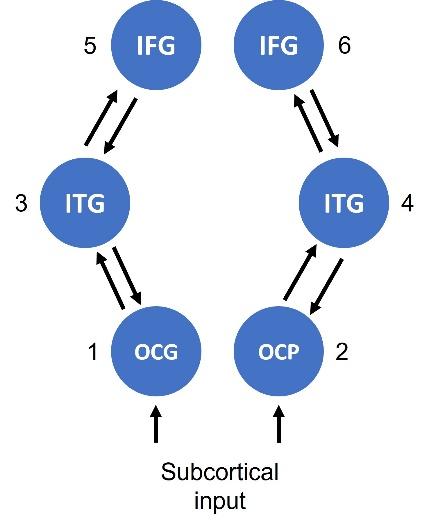
\includegraphics[width=1.94167in,height=2.39288in]{dcm_erp/figures/A_C_matrices.png}
\caption{\em Forward, backward connections and subcortical input, defined
in the A and C matrices in the neuronal model.\label{dcm-erp:fig:3}}
\end{center}
\end{figure}


\begin{figure}
\begin{center}
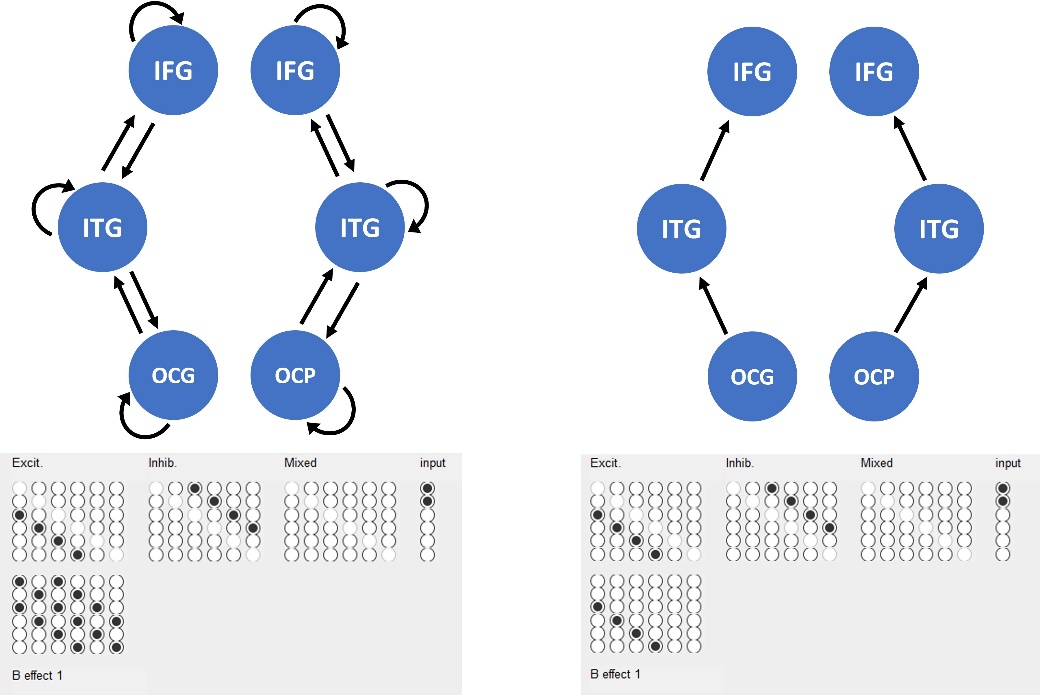
\includegraphics[width=4.73175in,height=3.15694in]{dcm_erp/figures/B_matrix.png}
\caption{\em Left: Model 1 with full B effect matrix, with modulatory
connections on both forward and backward connections, plus
self-connections. Right: Model 2 with reduced B effect matrix, with
modulatory connections only on forward connections.\label{dcm-erp:fig:4}}
\end{center}
\end{figure}

At the bottom of this section there are some additional options for the
model. The first option is 'dipolar symmetry constraints'; these can be
used as a prior on the model if you want to model bilateral sources.
This imposes a symmetry prior, and you can then run a model comparison
between models either with or without this dipolar symmetry prior
selected and examine the model fits between these two options. The
second option, 'optimise source locations', allows you to relax zero
variance priors on your specified source locations. The third option,
'lock trial-specific effects', enables you to enforce all trial-specific
coupling gains to be the same, and the final option, 'trial-specific
inputs', imposes trial-specific C parameter estimation.

\section{Estimation and Results}

Once you have completed the specification of your model, click `Invert'.
Starting the DCM model inversion opens a second graphics window. At the
top of the window you can see the hidden states of the two conditions:
on the left hand side is the first condition, the novel image condition,
and on the right hand side is the second condition, the repeated image
condition.

In this plot there is one line for each cell subpopulation for each
source in the model that we've specified, and this displays the hidden
source dynamics within the model. In the centre panel, the predicted and
observed responses are displayed in the principal component space or the
mode space. Here, the dotted lines represent the real observed data and
the solid lines represent the predicted response, and this is displayed
for each of the 8 modes that were defined in the model.

At the bottom of the window are the conditional model parameters: on the
left the conditional model parameters of the hidden states are shown,
and on the right the conditional model parameters of the forward model
(or observation model) are plotted.

During estimation, the main \matlab\ command window shows the number of
expectation-maximisation iterations that the model runs through
throughout the inversion. It also displays the predicted change and
actual change of free energy (\emph{F}) following each iteration step.
Once the model has fully estimated, SPM saves the results of the
inversion in a DCM file, named DCM\_*.mat, where * indicates the name of
the original EEG data file specified for the model. At the bottom left
of the DCM window there is a drop-down menu, which contains different
options through which to view your results.

\subsection{ERP (modes)}

By selecting 'ERP modes', you can see the eight different modes, i.e.
the essential principal components that are represented in the data. In
these plots, dotted lines represent the observed data, and solid lines
represent the model predictions, with different line colours indicating
the different task conditions. In this example, most of the data has
been captured within the first six or seven modes, so as an exercise,
one could define and invert a similar model for the same data using
fewer modes.

\subsection{ERP (sources)}

There is also the option to look at ERPs in source space. By selecting
this option, the graphics window shows one plot for each of the six
different sources as defined in our model. Each plot contains three
different dash patterns of lines representing the three different cell
subpopulations: population number one being the excitatory spiny
stellates, population two being inhibitory interneurons, and population
three are excitatory pyramidal cells. As above, different coloured lines
are used to indicate the different task conditions.

\subsection{Coupling (A)}

To look at the estimated values for the coupling between sources, click
`Coupling (A)'. This shows the conditional means of the estimates of the
coupling strengths as defined in our A matrices -- the matrices in which
we defined the forward, backward and lateral connections within the
model. This also shows the posterior probabilities, i.e. how likely
these estimates are given the observed data.

\subsection{Coupling (B)}

Similar to the above, by clicking `Coupling (B)' you can observe the
estimated values and posterior probabilities for between-source coupling
with the effect of task modulation, as defined earlier when setting up
the B effect matrix(es) for the model.

\subsection{Coupling (C)}

Similar to `Coupling (A)' and `Coupling (B)', but in this case you can
view the estimated values and posterior probabilities for inputs into
the sources specified in the input vector to receive subcortical input.

\subsection{Trial-specific Effects}

This option displays bar plots representing the estimated connection
strengths (\%) and direction of modulating effects for each connection
specified in the neuronal model, for each trial condition.

\subsection{Input}

By clicking `Input', you can see the estimated input function: this is a
gamma function with the addition of low-frequency terms.

\subsection{Response, and Response (image)}

The `Response' option plots the data selected by the spatial modes
defined in the model, back-projected into sensor space. Here you can
view the (adjusted) observed data and the model predictions for each of
the task conditions.

In the Response (image) option, you can see the same as with `Response',
but represented as a grey-scale image.

\subsection{Scalp Maps}

This displays the EEG scalp maps at different intervals across the time
window as specified in the `\emph{Data and Design}' part of the model
specification. Scalp maps are displayed for each task condition, for
both observed data and model predictions.

\subsection{Dipoles}

By clicking `Dipoles', you can view the locations of each source
specified in the `\emph{Electromagnetic Model}' section of model
specification. This option is only useful if you have selected ECD for
the spatial model, therefore this option is not available for this
example using IMG.

\section{Bayesian Model Comparison}

Now that you have successfully inverted your DCM, you can compare this
with an alternative model of the same data. You must ensure that the
first DCM you created is saved under a different name to the default;
click the `Save' button to rename the DCM file to make sure you don't
overwrite the file with the alternative model. To create an alternative
model for this example, return to the `\emph{Neuronal Model'} section in
the DCM window and edit the B effect matrix so that modulatory
connections are only present on the forward connections (\ref{dcm-erp:fig:4}).
To invert the new model, click `Estimated', ensuring that you do
not use the previous posterior or prior estimates. Once the alternative
model has been inverted, you can conduct Bayesian Model Comparison.

Click the `BMS' button at the bottom of the DCM window, and this will
open the batch editor for Bayesian Model Selection. You can also access
this by returning to the SPM GUI, and clicking `Batch' at the bottom.
This will open an empty batch editor window. Click `SPM' at the top,
then DCM \textgreater{} Bayesian Model Selection \textgreater{} Model
Inference. First, click `Directory' and specify the directory in which
the BMS output file will be saved. Click `Data', then `New Subject',
then `New Session'. Click `Models', and then click `Specify': you can
now select the DCM files in the file explorer for the two models you
wish to compare. It is important to remember the order in which you
select the DCM files; if you are comparing models across multiple
subjects, the DCM files should be selected in the same order for every
subject and session. If you wish to compare models for multiple
subjects, you would click `New Subject' for as many subjects you are
analysing and select the DCMs for that subject.

Select `Inference Method' and click Fixed Effects (FFX), as in this
example there are data and models for only one subject. Finally, click
the green `Run' arrow at the top to run the model comparison. The
graphics window now displays two bar plots (\ref{dcm-erp:fig:5}). The
top plot shows the log-model evidence of the two models you have
compared. The bottom plot shows the posterior probability for each
model, given the data. A model is generally judged to be the best model
for a given dataset compared with other models if its log-model evidence
is greater than the log-model evidences of competing models by at least
3.

\begin{figure}
\begin{center}
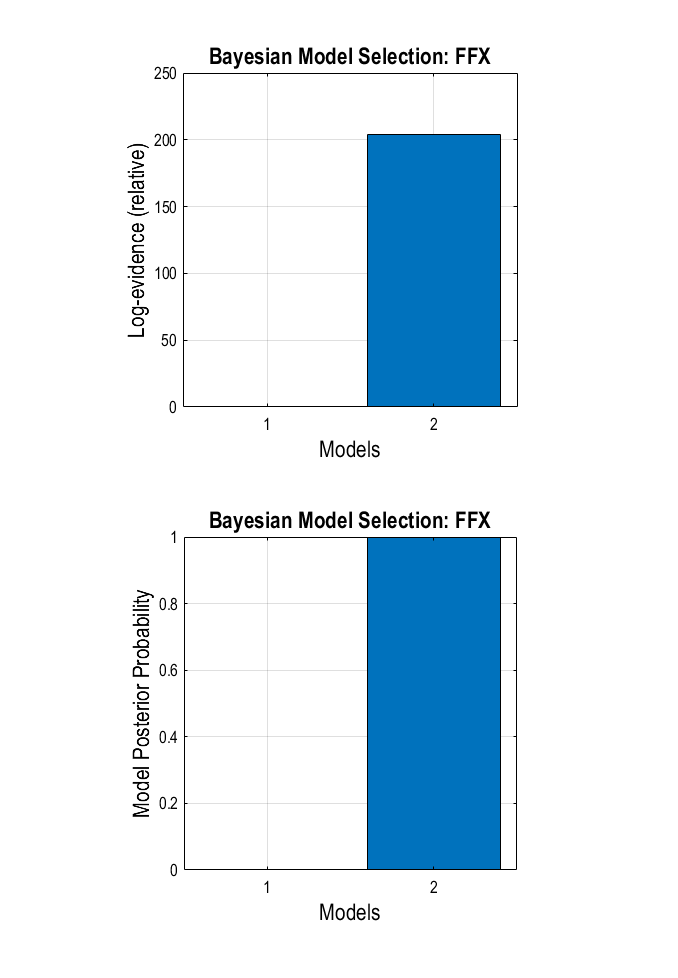
\includegraphics[width=3.36083in,height=6.93814in]{dcm_erp/figures/BMC.png}
\caption{\em Bayesian Model Comparison of the two models: the full B
matrix model (model 1) and the partial B matrix model (model 2). The
log-model evidence of model 2 is significantly higher than that of model
1 (log-model evidence is higher by more than 3), therefore model 2 is
the best model for this dataset.\label{dcm-erp:fig:5}}
\end{center}
\end{figure}

\section{References}

Moran RJ, Stephan KE, Dolan RJ, Friston KJ. Consistent spectral
predictors for dynamic causal models of steady-state responses.
Neuroimage 2011; 55: 1694-708.

Tyrer A, Gilbert JR, Adams S, Stiles AB, Bankole AO, Gilchrist ID\emph{,
et al.} Lateralized memory circuit dropout in alzheimer's disease
patients. Brain Commun 2020; 2: fcaa212.
